\documentclass[11pt]{article}
\usepackage{geometry}                % See geometry.pdf to learn the layout options. There are lots.
\geometry{a4paper}                   % ... or a4paper or a5paper or ... 
%\geometry{landscape}                % Activate for for rotated page geometry
%\usepackage[parfill]{parskip}    % Activate to begin paragraphs with an empty line rather than an indent
\usepackage{graphicx}
\usepackage{amssymb}
\usepackage{amsmath}
\usepackage{lipsum}
\usepackage{authblk}
\usepackage{bbold}
\usepackage{listings}
%\usepackage{amsaddr}
\usepackage{bm}
\usepackage{epstopdf}
\usepackage{booktabs}
\usepackage{xcolor}
\usepackage{fancyhdr}
\usepackage[yyyymmdd,hhmmss]{datetime}
\pagestyle{fancy}
\rfoot{Compiled on \today\ at \currenttime}
\cfoot{}
\lfoot{Page \thepage}
\RequirePackage[colorinlistoftodos,prependcaption,textsize=tiny]{todonotes} % look for '\todo'
\definecolor{darkred}{rgb}{0.4,0.0,0.0}
\definecolor{darkgreen}{rgb}{0.0,0.4,0.0}
\definecolor{darkblue}{rgb}{0.0,0.0,0.4}
\usepackage[bookmarks,linktocpage,colorlinks,
    linkcolor = darkred,
    urlcolor  = darkblue,
    citecolor = darkgreen]{hyperref}

%\DeclareGraphicsRule{.tif}{png}{.png}{`convert #1 `dirname #1`/`basename #1 .tif`.png}

\renewcommand{\headrulewidth}{0pt}
\fancyhead[L]{
%\includegraphics[width=4cm]{/Users/tomluu/Research/talks/fzjTemplate/uniBonn_logo.jpg}
}
\fancyhead[R]{
%\includegraphics[width=4cm]{/Users/tomluu/Research/talks/fzjTemplate/fzj_logo.jpg}
}
\pagestyle{plain}

\title{Simple documentation on \texttt{quboIsingHMC} code}
\author[1]{Jason Chang}
\author[1]{Christopher K\"orber}
\author[2,3]{Thomas Luu}
\author[3]{Johann Ostmeyer}
\affil[1]{LBL, Berkeley, California}
\affil[2]{Institute for Advanced Simulation 4\\
Forschungszentrum J\"ulich, Germany}
\affil[3]{HISKP, Rheinische Friedrich-Williams-Universit\"at Bonn, Germany}

%\email{t.luu@fz-juelich.de}
\date{}                                           % Activate to display a given date or no date


\begin{document}
\maketitle
\begin{center}
email: \href{mailto:t.luu@fz-juelich.de}{t.luu@fz-juelich.de}
\end{center}
\abstract{
Simple documentation for \texttt{quboIsingHMC} package.
}

\thispagestyle{fancy}

\clearpage{}
%\tableofcontents
%\newpage

\section{Running the code}
The codes are in the \texttt{src} directory.  Modify the \texttt{Makefile} to point to your relevant \texttt{C++} compiler.  The relevant files are 
\begin{itemize}
\item \texttt{quboIsingHMC.h} contains the necessary declarations.
\item \texttt{quboIsingHMC.cpp} contains the codes for HMC and measurements.
\item \texttt{anneal.cpp} is the driver that does simple annealing.  Modify this file (or make a new one) to change the parameters $\beta$, mass parameter $\mathcal{C}$ (described in the next section), number of thermalizations, number of measurements, etc. . .  Hopefully I commened this file enough for you to understand what's going on, and more importantly, to change it yourself.
\item \texttt{input\_KandH.dat} is the input file that has the simple toy problem.  Modify this file (or make a new one) to investigate some other graph system.  It's pretty self-explanatory.
\end{itemize}
Just type ``make" and the \texttt{Makefile} will make the executable \texttt{anneal.exe}.  To run this executable, enter
\begin{lstlisting}
./anneal.exe input_KandH.dat > output.dat
\end{lstlisting}
Here the results are piped into the \texttt{output.dat} file.  Once you have produced results in the \texttt{output.dat} file, you can also run
\begin{lstlisting}
python3 histPsi.py output.dat
python3 bootstrapData.py output.dat
\end{lstlisting}
The first will plot out a histogram of the $\langle\psi\rangle$ fields.  The second will attempt to get errors on $\langle E\rangle$, $\langle m\rangle$, and individual $\langle s_i\rangle$.  These are just my own personal routines to get some quick and dirty statistics and to see what's going on.  I'm sure you have more sophisticated routines. An example output from running \texttt{bootstrapData.py} is
{\tiny
\begin{lstlisting}
# <E>     <dE>       <m>        <dm>
1.53701004750845   0.039486985506858106   -0.47805792873174674   0.0015377626813233474

# i   <S_i>     <dS_i>
1   -0.22137956326262076   0.006769260613688914
2   0.25949543710881184   0.006664269745196156
3   -0.27070330907695045   0.006751158852773441
4   -0.8892316241971162   0.0026959779928807403
5   -0.24806636360105197   0.005744952355068994
6   -1.0039863533419193   0.005359143190295709
7   -0.9725337094797504   0.002067991089669495
\end{lstlisting}}\noindent
An example output from \texttt{histPsi.py} is shown in \autoref{fig:histPsi}.
\begin{figure}
\center
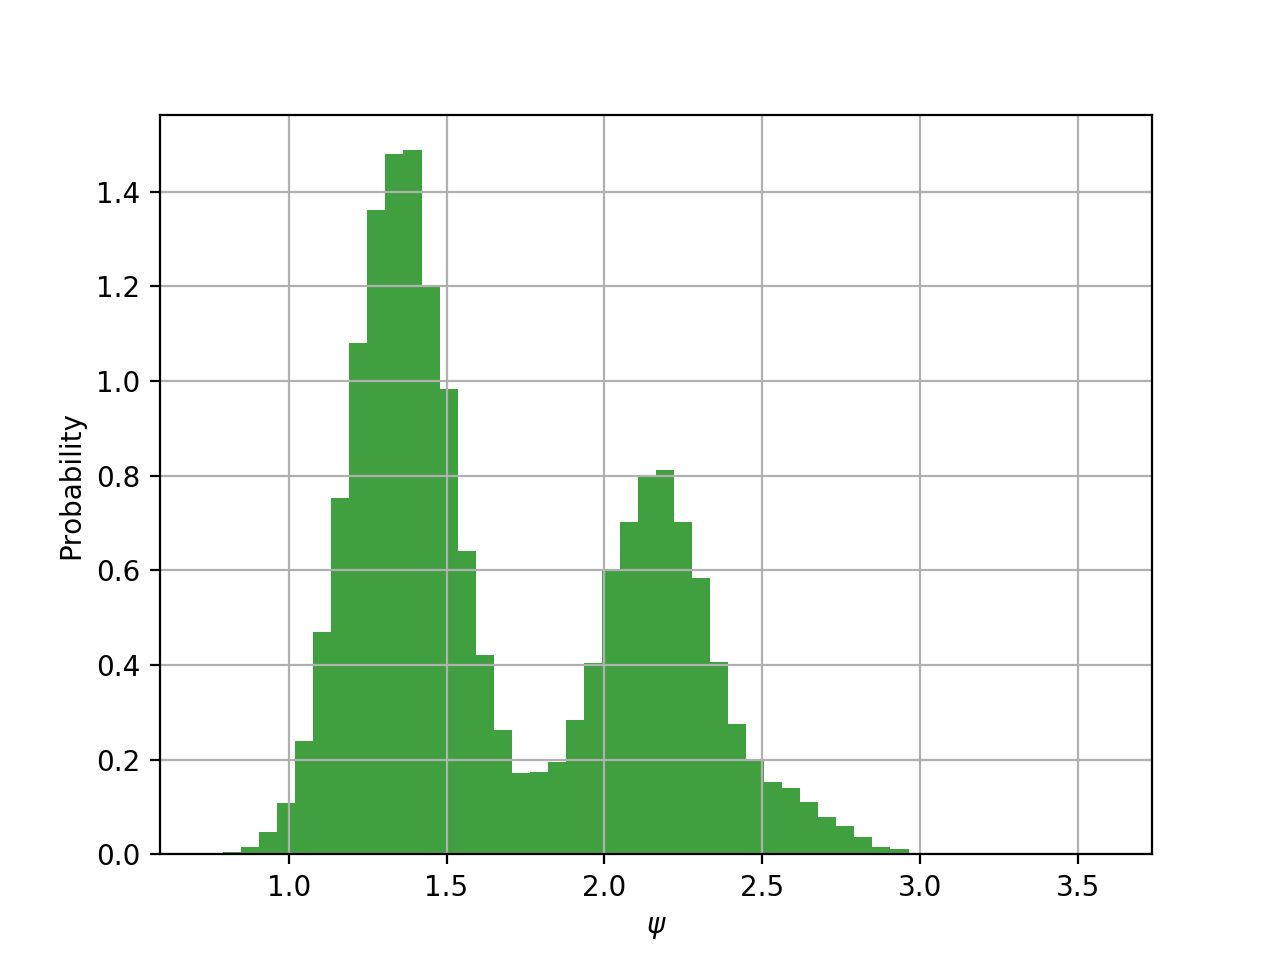
\includegraphics[width=.8\columnwidth]{figures/histPsi.png}
\caption{Example of histogram of average HS auxialiary field, $\langle \psi\rangle$. \label{fig:histPsi}}
\end{figure}

\section{Simple test problem}
The Hamiltonian is\footnote{Note that the signs in front of $s_iK_{ij}s_j$ and $h_is_i$ are opposite of Jason's and Christopher's convention.}  
\begin{align}
H[\bm s]&=-\sum_{ij}s_iK_{ij}s_j-\sum_ih_is_i+\mathcal{E}\label{eqn:H1}\\
&=-\bm s^{\rm T}K\bm s-\bm h^{\rm T}\bm s+\mathcal{E}\ ,
\end{align}
where the spins $s_i=\pm 1$, $\mathcal{E}=23/2$, 
\begin{equation}
\bm h = \begin{pmatrix}
5/2\\ 7/2\\ 5/2\\  -1\\  -2\\  -4 \\  -1
\end{pmatrix}\ ,
\end{equation} 
and
\begin{equation}\label{eqn:K}
K=
\begin{pmatrix}
 0&  -2&  -1& 1& 1& 2&  0\\
         0&  0&  -2& 1& 1& 2& 1	\\
         0&  0&  0&  0& 1& 2& -1\\
         0&  0&  0&  0&  0&  0&  0\\
         0&  0&  0&  0&  0&  -2&  0\\
         0&  0&  0&  0&  0&  0&  0\\
         0&  0&  0&  0&  0&  0&  0
        \end{pmatrix}\ .
        \end{equation}
A brute force scan of the phase space shows that the minimum energy occurs when
\begin{equation}
\bm s=\begin{pmatrix}
-1\\ 1\\ -1\\ -1\\ -1\\ -1\\ -1
\end{pmatrix}\quad,\quad H[\bm s]=1\implies \epsilon = \frac{1}{7}\quad, m = -\frac{5}{7}\ ,
\end{equation}
where $\epsilon$ and $m$ are the average energy and magnetization per site, respectively. 
\begin{figure}
\center
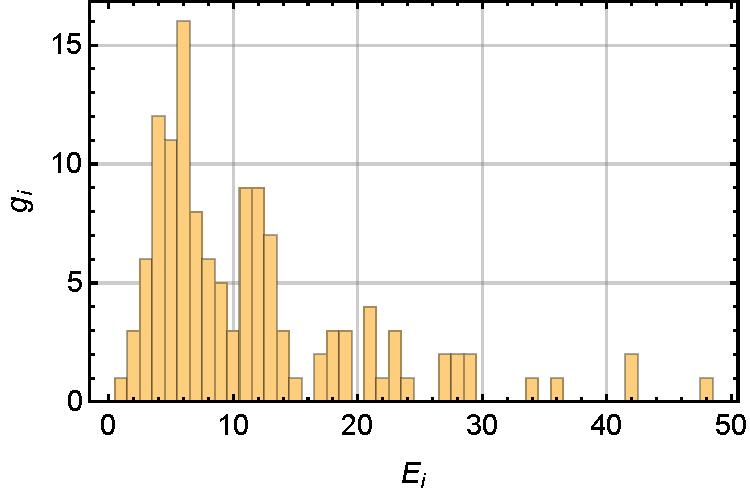
\includegraphics[width=.8\columnwidth]{figures/histogram.pdf}
\caption{Energy states $E_i$ and degeneracy $g_i$ for Hamiltonian defined in Eqs.~\eqref{eqn:H1}-\eqref{eqn:K}.\label{fig:histogram}}
\end{figure}


\section{Applying the HS transformation}
The first thing we do is symmetrize the connectivity matrix, 
\begin{equation}
-\bm s^{\rm T}K\bm s =-\frac{1}{2}\bm s^{\rm T}\left(K^{}+K^{\rm T}\right)\bm s\equiv-\frac{1}{2}\bm s^{\rm T}K_{\rm sym}\bm s\ .
\end{equation}
Now the eigenvalues of $K_{\rm sym}$ are
\begin{align*}
\lambda_i = \{&2.70601700045421, 2.46355010284599, 1.61803398874989, \\
&1.19404817052648, -0.593828775261607, -0.618033988749895,\\ 
-&6.76978649856507\}\ .
\end{align*}
To ensure that the Hubbard-Stratonovich transformation is stable, we add a mass term $\mathcal{C}$ to $K_{\rm sym}$,
\begin{equation}
\tilde K \equiv K_{\rm sym}+\mathcal{C}\mathbb{1}_7\ ,
\end{equation}
where $\mathcal{C}> 6.76978649856507$.  The eigenvalues of the symmetric matrix $\tilde K$ are now all positive definite.  Using the fact that $s_i^2=1\ \forall\  i$ we can compensate for this mass by an overall shift in the Hamiltonian,
\begin{equation}
H[\bm s]=-\frac{1}{2}\bm s^{\rm T}\tilde K\bm s-\bm h^{\rm T}\bm s+\mathcal{E}+\frac{7}{2}\mathcal{C}\ .
\end{equation}

\subsection{The partition function $\mathcal{Z}$}
The partition function is
\begin{equation}
\mathcal{Z}=\sum_{\{s_i=\pm 1\}}e^{-\beta H[\bm s]}=e^{-\beta\mathcal{E}-\frac{7}{2}\beta\mathcal{C}}
\sum_{\{s_i=\pm 1\}}e^{\frac{1}{2}\beta\bm s^{\rm T}\tilde K\bm s+\beta\bm h^{\rm T}\bm s}
\end{equation}
Now apply the HS transformation for each site,
\begin{equation}
\mathcal{Z}=e^{-\beta\mathcal{E}-\frac{7}{2}\beta\mathcal{C}}
\sum_{\{s_i=\pm 1\}}\int_{-\infty}^{\infty} \frac{1}{\sqrt{\operatorname{det} \tilde{K}}}\left[\prod_{i} \frac{d \phi_{i}}{\sqrt{2 \pi \beta}}\right] e^{-\frac{1}{2 \beta} \sum_{i j} \phi_{i} \tilde{K}_{i j}^{-1} \phi_{j}+\sum_{i} s_{i}\left(\beta h_i+\phi_{i}\right)}\ .
\end{equation}
We can now ``integrate out the spins",
\begin{align}
\mathcal{Z}&=e^{-\beta\mathcal{E}-\frac{7}{2}\beta\mathcal{C}}
\int_{-\infty}^{\infty} \frac{1}{\sqrt{\operatorname{det} \tilde{K}}}\left[\prod_{i} \frac{d \phi_{i}}{\sqrt{2 \pi \beta}}\right] \sum_{\{s_i=\pm 1\}}e^{-\frac{1}{2 \beta} \sum_{i j} \phi_{i} \tilde{K}_{i j}^{-1} \phi_{j}+\sum_{i} s_{i}\left(\beta h_i+\phi_{i}\right)}\\
&=e^{-\beta\mathcal{E}-\frac{7}{2}\beta\mathcal{C}}
\int_{-\infty}^{\infty} \frac{1}{\sqrt{\operatorname{det} \tilde{K}}}\left[\prod_{i} \frac{d \phi_{i}}{\sqrt{2 \pi \beta}}\right] e^{-\frac{1}{2 \beta} \sum_{i j} \phi_{i} \tilde{K}_{i j}^{-1} \phi_{j}}\left[\prod_i 2\cosh\left(\beta h_i+\phi_{i}\right)\right]\\ 
&=\frac{e^{-\beta\mathcal{E}-\frac{7}{2}\beta\mathcal{C}}}{\sqrt{\operatorname{det} \tilde{K}}}
\int_{-\infty}^{\infty}\left[\prod_{i} \frac{d \phi_{i}}{\sqrt{2 \pi \beta}}\right] e^{-\frac{1}{2 \beta} \sum_{i j} \phi_{i} \tilde{K}_{i j}^{-1} \phi_{j}+\sum_i\log\left(2\cosh\left(\beta h_i+\phi_{i}\right)\right)}\
\end{align}
We're almost there.  Now make the change of variables,
\begin{equation}
\phi_{i}=\sqrt{\beta}\tilde{K}_{i j} \psi_{j}-\beta h_{i}\ .
\end{equation}
Ok, we'll skip a couple of steps now, but it's relatively straightforward to make the substitution above and obtain the final version of the partition function in terms of the field $\psi$,
\begin{multline}\label{eqn:Z}
\mathcal{Z}=e^{-\beta\mathcal{E}-\frac{7}{2}\beta\mathcal{C}}\sqrt{\operatorname{det}\tilde K}e^{-\frac{1}{2} \beta \bm h^{\rm T} \tilde{K}^{-1} \bm h}\\
\int_{-\infty}^{\infty}\left[\prod_{i} \frac{d \psi_{i}}{\sqrt{2 \pi}}\right]
e^{-\frac{1}{2}\bm\psi^{\rm T} \tilde K\bm \psi+\sqrt{\beta}\bm h^{\rm T}\bm\psi+\sum_i\log\left\{2\cosh\left(\sqrt{\beta}\left[\tilde{K}\bm \psi\right]_i\right)\right\}}\\
\equiv e^{-\beta\mathcal{E}-\frac{7}{2}\beta\mathcal{C}}\sqrt{\operatorname{det}\tilde K}e^{-\frac{1}{2} \beta \bm h^{\rm T} \tilde{K}^{-1} \bm h}
\int\mathcal{D}[\bm\psi]
e^{-S[\bm\psi]}\ ,
\end{multline}
where
\begin{equation}
S[\bm\psi]=\frac{1}{2}\bm\psi^{\rm T} \tilde K\bm \psi-\sqrt{\beta}\bm h^{\rm T}\bm\psi-\sum_i\log\left\{2\cosh\left(\sqrt{\beta}\left[\tilde{K}\bm \psi\right]_i\right)\right\}\ .
\end{equation}
The form of this expression is convenient since the only place where an inverse shows up is in $\beta \bm h^{\rm T} \tilde{K}^{-1} \bm h$ and this term is independent of the field $\psi$.  Even though this term does not impact the force equations in HMC, we still need it for obtaining the mean energy (and other quantities) when $h_i\ne 0$.  This will be more clear in the next subsections.  At the beginning of any calculation one can solve the linear equation (just once)
\begin{displaymath}
\tilde K\bm\kappa =\bm h\implies \bm \kappa = \tilde K^{-1}\bm h\ ,
\end{displaymath}
which allows the replacement
\begin{displaymath}
\beta \bm h^{\rm T} \tilde{K}^{-1} \bm h\rightarrow\beta \bm h^{\rm T}\bm \kappa\ .
\end{displaymath}
Finally, we define 
\begin{equation}
\langle \kappa\rangle =\frac{1}{\Lambda}\sum_i\kappa_i\ .
\end{equation}

\subsection{$\langle E\rangle$}
The extensive energy is given by
\begin{align}
\langle E\rangle&=-\frac{\partial}{\partial \beta} \log (\mathcal{Z})\label{eqn:energy}\\
&\equiv\frac{\int\mathcal{D}[\bm\psi]\ O_{\langle E\rangle}[\bm\psi]e^{-S[\bm\psi]}}{\int\mathcal{D}[\bm\psi]e^{-S[\bm\psi]}}\ .
\end{align}
Plugging~\eqref{eqn:Z} into~\eqref{eqn:energy} one finds
\begin{equation}\label{eqn:energy op}
O_{\langle E\rangle}[\bm\psi]=\mathcal{E}+\frac{\Lambda\mathcal{C}}{2}
+\frac{1}{2}\bm h^{\rm T}\bm\kappa
-\frac{1}{2\sqrt{\beta}}\bm h^{\rm T}\bm\psi
-\frac{1}{2 \sqrt{\beta}} \sum_{i} [\tilde{K}\bm\psi]_i \tanh \left(\sqrt{\beta} [\tilde{K}\bm\psi]_i\right)\ ,
\end{equation}
where $\Lambda$ is the total dimension of the system  (here $\Lambda=7$). 
It is convenient here, and later, to define
\begin{equation}
\bm\varphi = \tilde K\bm \psi\ ,
\end{equation}
which means eq.~\eqref{eqn:energy op} becomes
\begin{equation}\label{eqn:energy op2}
O_{\langle E\rangle}[\bm\psi]=\mathcal{E}+\frac{\Lambda\mathcal{C}}{2}
+\frac{1}{2}\bm h^{\rm T}\bm\kappa
-\frac{1}{2\sqrt{\beta}}\bm h^{\rm T}\bm\psi
-\frac{1}{2 \sqrt{\beta}} \sum_{i} \varphi_i \tanh \left(\sqrt{\beta} \varphi_i\right)\ .
\end{equation}
The subroutine that calculates this quantity is in \texttt{quboIsingHMC.cpp}:
{\tiny
\begin{lstlisting}
double ising::calcE(){
  // calculates energy

  E1 =  mathcalE + Lambda*C/2.;
  for (int i=0;i< Lambda; i++)
    E1 +=  h[i]*k[i]/2. - h[i]*psi[i]/2./sqrtBeta - varphi[i]*tanh(sqrtBeta*varphi[i])/2.0/sqrtBeta;
  return E1;
    
}
\end{lstlisting}
}

\subsection{Average magnetization}
The average magnetization is given by
\begin{align}
\langle m\rangle&=\frac{1}{\Lambda \beta}\sum_i \frac{\partial}{\partial h_i} \log (\mathcal{Z})\\
&\equiv\frac{\int\mathcal{D}[\bm\psi]\ O_{\langle m\rangle}[\bm\psi]e^{-S[\bm\psi]}}{\int\mathcal{D}[\bm\psi]e^{-S[\bm\psi]}}\ .
\end{align}
As was done in the previous section, one just has to take derivatives, but now with respect to $h_i$.  A little work gives
\begin{align}
O_{\langle m\rangle}[\bm\psi]&=\frac{1}{\sqrt{\beta}}\frac{1}{\Lambda}\sum_i\psi_i -\frac{1}{\Lambda}\sum_i\kappa_i\nonumber\\
&=\frac{1}{\sqrt{\beta}}\frac{1}{\Lambda}\sum_i\psi_i -\langle \kappa\rangle\ .\label{eqn:m op}
\end{align}
The subroutine that calculates this quantity is in \texttt{quboIsingHMC.cpp}:
\begin{lstlisting}
double ising::calcM(){
  // calculates magnetization

  M1 = mean(psi,Lambda)/sqrtBeta - kappa;
  return M1;

}
\end{lstlisting}

\section{HMC}
The artificial Hamiltonian is
\begin{equation}
\mathcal{H}[\bm p,\bm \psi]=\frac{\bm p^2}{2}+S[\bm \psi]\ .
\end{equation}
The force equations are (repeated indices are summed)
\begin{equation}
\begin{array}{l}
{\dot{\psi_i}=\frac{\partial \mathcal{H}}{\partial p_i}=p_i} \\
{\dot{p_i}=-\frac{\partial \mathcal{H}}{\partial\psi_i}=-\tilde{K}_{ij} \psi_j+\sqrt{\beta}h_i+\sqrt{\beta} \tilde{K}_{ij} \tanh (\sqrt{\beta} \tilde{K}_{jk} \psi_k)}\\
{\quad\ =-\varphi_i+\sqrt{\beta}h_i+\sqrt{\beta} \tilde{K}_{ij} \tanh (\sqrt{\beta} \varphi_j)}\ .
\end{array}
\end{equation}
We use $\bm \varphi=\tilde K\bm \psi$ in the last line above. No matrix inversion anywhere!   The calculation of the forces is done in \texttt{quboIsingHMC.cpp}, in the subroutine
{\tiny
\begin{lstlisting}
int ising::calcPdot(){

  sprsax(var,rld,psi,varphi2,Lambda);  // this gives varphi2[i] = K[i][j]*psi[j]
  for(int i=0; i < Lambda; i++)  // this makes the vector varphi3[i] = sqrtBeta*tanh(sqrtBeta*K[i][j]*psi[j])
    varphi3[i]=sqrtBeta*tanh(sqrtBeta*varphi2[i]);
  sprsax(var,rld,varphi3,pdot,Lambda); // this gives pdot[i] = sqrtBeta*K[i][j]*tanh(spqrtJ*varphi2[j])
  for(int i=0; i < Lambda; i++)
    pdot[i] += -varphi2[i] + h[i]*sqrtBeta;

  return 0;
}
\end{lstlisting}
}

\section{Ergodicity}
Actually, it's most likely we \emph{do not} want to fix any ergodicity problem.  We want the solution to fall into certain minima.  We can always re-heat and cool down again and see if we fall into any lower energy solution.  But it's good to explain what type of ergodicity problems there are with this formalism. . .
%\newpage
%\appendix

%\clearpage
%\bibliography{references}

\end{document}  
